% questions.tex —— 1977 年·甘肃卷 · 题目内容片段（无答案）
% 由 tools/generate_projects.py 依来源总账自 1977/1977_数学真题_甘肃_试题.md 生成，勿手改（改源 MD 后重跑）


\gkpart{数学试题解（甘肃卷）}

\begin{gktip}
\textbf{来源说明}：本题面依据固定源 PDF《甘肃1977年高考数学试题解》第 1—4 页逐题转录。源卷为题面与解答连续排印的《试题解》材料（第 1—8 题），不是纯题面卷；未附文理分科说明，全卷不分文理，无附加题或参考题。源 PDF 页面底部印有书籍页码 118—121，本文按 PDF 页序记录。第 5 题源卷附有编者注（见题后留注）；答案与解析由本库对照源解答独立复算。
\end{gktip}

\par\medskip

\begin{question}
\gkti{1}用“$>$”、“$<$”、“$=$”号分别把下列各组数连接起来：

（1） $0.25+3\dfrac{1}{8}$ 与 $|-3.375|$；

（2） $\left(\dfrac{\sqrt{3}}{3}-\dfrac{1}{\sqrt{3}}\right)^{3}$ 与 $(-3)^{0}$；

（3） $-\lg 0.01$ 与 $\log_4\dfrac{1}{16}$；

（4） $\operatorname{tg} 44^\circ$ 与 $\operatorname{ctg} 44^\circ$。

\end{question}
\begin{question}
\gkti{2}解答下列各题：

\Needspace{5\baselineskip}
（1） 计算：

\nopagebreak[4]
\[
\frac{2a}{a-3b}-\frac{6ab-24b^2}{a^2-7ab+12b^2}.
\]

\Needspace{5\baselineskip}
（2） 化简：

\nopagebreak[4]
\[
\frac{(a^{\frac{8}{5}}b^{-\frac{6}{5}})^{-\frac{1}{2}}\sqrt[5]{a^4}}{\sqrt[5]{b^3}}.
\]

\Needspace{5\baselineskip}
（3） 证明：

\nopagebreak[4]
\[
\frac{2\operatorname{ctg}x}{1+\operatorname{ctg}^2x}=\sin 2x.
\]

（4） 求函数 $y=\dfrac{1}{2}x^2+3x+9$ 的极值。

\Needspace{0.4\textheight}
\end{question}
\begin{question}
\gkti{3}$AD$ 是 $\triangle ABC$ 外接圆的直径，$AD=6$，$\angle DAC=\angle ABC$，求 $AC$（精确到 $0.01$）。
\nopagebreak[4]
\begin{center}% 1977 年甘肃卷第三题：△ABC 的外接圆，AD 为直径（A 右上、D 下偏左），
% 弦 AB、BC、CA 实线，辅助线 DC 虚线（源卷解答“连接CD”所加），
% ∠ABC（B 处）与 ∠DAC（A 处）画角弧（按源卷第 2 页布局）
\begin{tikzpicture}[scale=0.9]
  \coordinate (O) at (0,0);
  \coordinate (A) at (60:2);
  \coordinate (B) at (185:2);
  \coordinate (C) at (300:2);
  \coordinate (D) at (240:2);
  \draw[thick] (O) circle (2);
  \draw[thick] (A)--(B)--(C)--cycle;
  \draw[thick] (A)--(D);
  \draw[dashed] (D)--(C);
  \fill (A) circle (1.2pt) node[above right] {$A$};
  \fill (B) circle (1.2pt) node[left] {$B$};
  \fill (C) circle (1.2pt) node[right] {$C$};
  \fill (D) circle (1.2pt) node[below] {$D$};
  % ∠ABC 角弧：BA 方向约 32.5°，BC 方向约 -27.5°
  \draw ($(B)+({0.5*cos(-27.5)},{0.5*sin(-27.5)})$)
        arc[start angle=-27.5, end angle=32.5, radius=0.5];
  % ∠DAC 角弧：AD 方向 -120°，AC 方向 -90°
  \draw ($(A)+({0.55*cos(-120)},{0.55*sin(-120)})$)
        arc[start angle=-120, end angle=-90, radius=0.55];
\end{tikzpicture}
\end{center}
\nopagebreak[4]
\Needspace{0.4\textheight}
\end{question}
\begin{question}
\gkti{4}在 $\triangle ABC$ 中，$\angle A=30^\circ$，$\angle B-\angle C=60^\circ$，$BC=2$，求 $AC$（用根式表示）。
\nopagebreak[4]
\begin{center}% 1977 年甘肃卷第四题：△ABC（A 左下、B 上、C 右下），
% ∠A 处画角弧并标 30°，BC 边中段标边长 2（按源卷第 2 页布局）
\begin{tikzpicture}[scale=1.0]
  \coordinate (A) at (0,0);
  \coordinate (B) at (2.4,1.9);
  \coordinate (C) at (4.6,0);
  \draw[thick] (A)--(B)--(C)--cycle;
  \fill (A) circle (1.2pt) node[below left] {$A$};
  \fill (B) circle (1.2pt) node[above] {$B$};
  \fill (C) circle (1.2pt) node[below right] {$C$};
  % ∠A 角弧：AB 方向约 38.4°，AC 方向 0°
  \draw ($(A)+(0.7,0)$) arc[start angle=0, end angle=38.4, radius=0.7];
  \node at (1.15,0.28) {$30^\circ$};
  % BC 边长标注
  \node at (3.65,0.85) {$2$};
\end{tikzpicture}
\end{center}
\nopagebreak[4]
\end{question}
\begin{question}
\gkti{5}某生产队现已平整土地 $100$ 亩，计划两年后平整土地的总面积要在 $225$ 亩以上，求每年平均增长率。

\begin{gktip}
\textbf{源注}：源卷在此题题面后附有编者注，指出此题题意不清、无法按原题求解，并给出改动后的题意与解法；注文全文引录见解析正文。
\end{gktip}

\Needspace{0.4\textheight}
\end{question}
\begin{question}
\gkti{6}如图，右图的二视图表示什么形体？用直径为 $40$ 毫米的圆柱形钢材锻压这样一个工件，需截取多长一般钢材？

\begin{gktip}
\textbf{源注}：「一般」系源卷原文，按文义应为「一段」；原文「园柱」「园台」等用字已按今习惯写作「圆柱」「圆台」。
\end{gktip}
\nopagebreak[4]
\begin{center}% 1977 年甘肃卷第六题：圆台二视图（上：正视图等腰梯形，标 ∅20、∅60；
% 下：俯视图同心圆；竖直点划线为轴线，贯穿两视图，按源卷第 3 页布局）
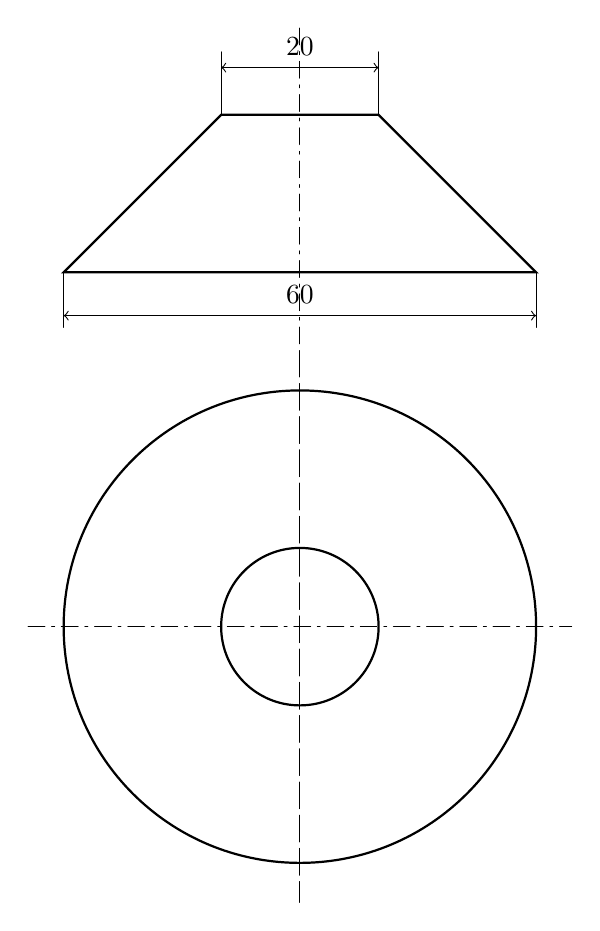
\begin{tikzpicture}[scale=0.5, line cap=round]
  % ---- 正视图：等腰梯形 ----
  \coordinate (TL) at (-2,13);
  \coordinate (TR) at (2,13);
  \coordinate (BR) at (6,9);
  \coordinate (BL) at (-6,9);
  \draw[thick] (TL)--(TR)--(BR)--(BL)--cycle;
  % 上口尺寸线 ∅20
  \draw[thin] (-2,13)--(-2,14.6);
  \draw[thin] (2,13)--(2,14.6);
  \draw[<->] (-2,14.2)--(2,14.2);
  \node[above] at (0,14.25) {$\varnothing 20$};
  % 下口尺寸线 ∅60
  \draw[thin] (-6,9)--(-6,7.6);
  \draw[thin] (6,9)--(6,7.6);
  \draw[<->] (-6,7.9)--(6,7.9);
  \node[above] at (0,7.95) {$\varnothing 60$};
  % ---- 竖直轴线（点划线，贯穿两视图）----
  \draw[dash pattern={on 6pt off 2.5pt on 1pt off 2.5pt}, thin]
        (0,15.2)--(0,-7);
  % ---- 俯视图：同心圆 ----
  \draw[thick] (0,0) circle (6);
  \draw[thick] (0,0) circle (2);
  \draw[dash pattern={on 6pt off 2.5pt on 1pt off 2.5pt}, thin]
        (-6.9,0)--(6.9,0);
  \draw[dash pattern={on 6pt off 2.5pt on 1pt off 2.5pt}, thin]
        (0,-6.9)--(0,7);
\end{tikzpicture}
\end{center}
\nopagebreak[4]
\end{question}
\begin{question}
\gkti{7}一条直线通过 $(3,0)$，并且和直线 $y=-2x+9$ 垂直，求这条直线与直线 $2y+5x=3$ 的交点的坐标。

\end{question}
\begin{question}
\gkti{8}

（1） 已知 $\dfrac{dy}{dy}=x\mathrm{e}^{x}+2\cos x+3x^2$，求 $y$；

\begin{gktip}
\textbf{源注}：源卷等式左端分母印作「$dy$」（即 $\dfrac{dy}{dy}$）；依源解答「在已知等式两边积分」的意图应为 $\dfrac{dy}{dx}$，解析正文按 $\dfrac{dy}{dx}$ 求解。
\end{gktip}

（2） 过点 $p(4,0)$ 向曲线 $x^2+y^2=1$ 作切线，求切线方程。


\end{question}